% Geometry, font
\documentclass[12pt, letter]{article}
\usepackage[margin=0.8in]{geometry}
\usepackage[T1]{fontenc}
\usepackage{fourier}
\usepackage{titling}
\setlength{\droptitle}{-5em} 
\usepackage[parfill]{parskip}
\usepackage{graphicx}
\graphicspath{{imgs/}}
\usepackage{hyperref}

% Math stuff
\usepackage{amssymb}
\usepackage{bm}

% Code Highlighting
\usepackage{minted}
\usemintedstyle{solarizedlight}

\author{Zach Neveu}
\title{ Day 6 Notes }

\begin{document}
\maketitle

\section{Review}%
\label{sec:review}
\begin{itemize}
	\item NPC proof via sub-problem (see Venn diagram from day 5)
	\item If sub-problem is NPC, problem is NPC
	\item If problem is P, sub-problem also P
	\item Sub-problems can be organized recursively (Complexity Landscape\textsuperscript{TM})
\end{itemize}
\begin{figure}[h]
	\centering
	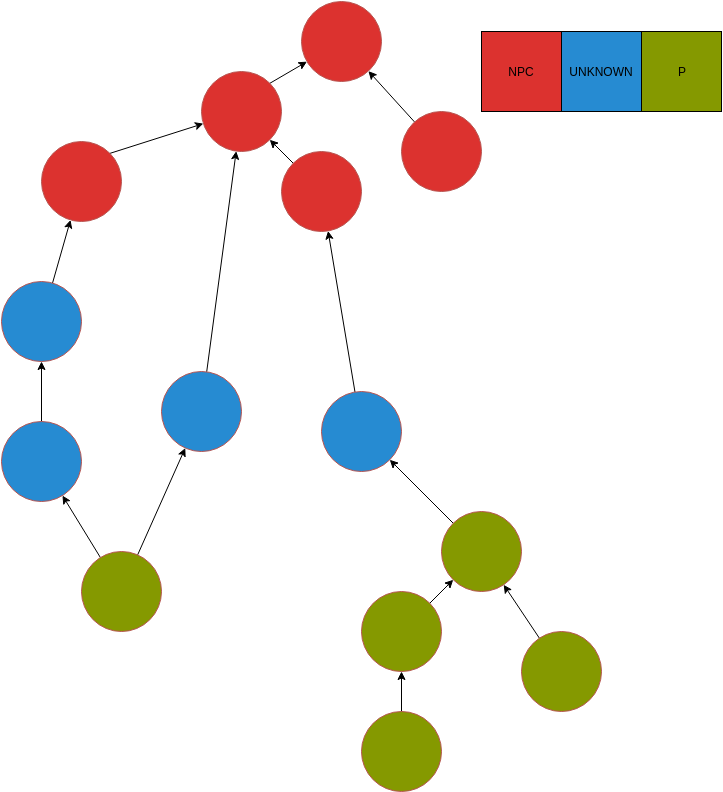
\includegraphics[width=0.8\textwidth]{complexity-landscape}
	\caption{Example Complexity Landscape\textsuperscript{TM}}
	\label{fig:complexity-landscape}
\end{figure}

\subsection*{Example: Procedure Constrained Scheduling (PCS)}
\begin{figure}[h]
	\centering
	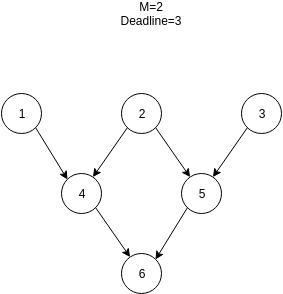
\includegraphics[width=0.4\textwidth]{schedule}
	\caption{Example PCS Constraint}
	\label{fig:schedule}
\end{figure}
\begin{itemize}
	\item Given a set of tasks that each take one unit of time to complete, a partial order on the tasks, a number, m, of processors, and an integer deadline
	\item Question: Does a legal schedule allow the processes to be completed before the deadline?
	\item General PCS $\in$ NPC
	\item If constraints graph is tree, $PCS \in P$
	\item If constraints graph empty, $PCS \in P$
	\item Aside: Why m=2 solvable, but m=3 so hard?
	\item Consider: 3 is important. 
	\item $2SAT \in P$, $3SAT \in NPC$, same for HC problem
\end{itemize}

\begin{figure}[h]
	\centering
	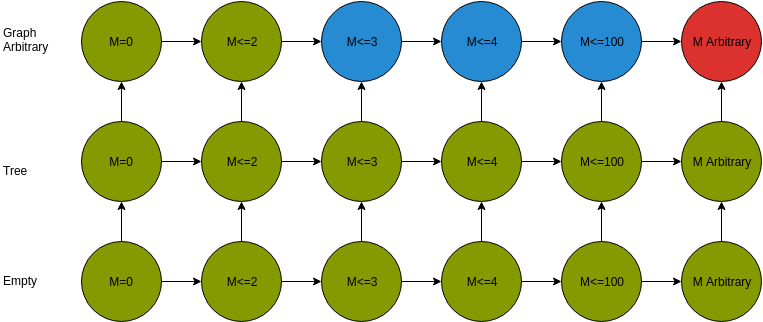
\includegraphics[width=0.8\textwidth]{schedule-landscape}
	\caption{PCS Complexity Landscape\textsuperscript{TM}}
	\label{fig:schedule-landscape}
\end{figure}

\subsection*{Special Nodes}
A node on the Complexity Landscape that has no known NPC children is called \textbf{Minimally NPC}  \\
A node on the Complexity Landscape that is in P and has no parents in P is called \textbf{Maximally polynomially solvable} 

\section{Greedy Algorithms}%
\label{sec:greedy_algorithms}
\begin{itemize}
	\item A \textbf{Greedy Algorithm} always makes what appears to be the best decision in the current moment
	\item A \textbf{Greedy Algorithm} does not utilize backtracking
\end{itemize}

\subsection*{MST}
MST: Given an undirected graph and a weight for each edge, find an acyclic subset of the edges that connects all nodes with minimum weight.

\begin{minted}[mathescape]{Python}
def MST():
  A=0
  while A is not spanning tree:
    find next edge (u,v) in increasing order by weight such that (u,v) is safe for A
    A += {(u,v)}
  return A
\end{minted}

\subsection*{Activity Selection}
\begin{itemize}
	\item Given: a set $S=\{a_1, a_2, \ldots, a_n\}$ of n activities, only one of which can take place at a time. Activity $a_i$ starts at time  $s_i$ and finishes at time $f_i$. Two activities are \textbf{Compatible} if they do not conflict.
	\item Find: How many activities can we fit?
	\item Find a largest set of mutually compatible activities
\end{itemize}

\begin{table}
\begin{center}
\begin{tabular}{|c|c|c|c|c|c|c|c|c|c|c|c|}
\hline
# & 1 & 2 & 3 & 4 & 5 & 6 & 7 & 8 & 9 & 10 & 11 \\
\hline
$s_i$ & 1 & 3 & 0 & 5 & 6 & 8 & 8 & 2 & 12 & 3 & 5 \\
\hline
$f_i$ & 4 & 5 & 6 & 7 & 10 & 11 & 12 & 13 & 14 & 8 & 9 \\
\hline
\end{tabular}
\end{center}
\caption{Example Activity Problem}
\end{table}

\begin{minted}{Python}
# Solution
# a[i] is most recently selected activity
# a[m] activity we are considering adding
def activitySelection(a):
  sortByIncreaseFinish(a)
  n = number of Activities
  A = a[0] # first activity
  i = 1
  for m in range(1,n):
    if not conflict(a[m], a[i]):
      A += a[m]
      i = m
  return A
\end{minted}

\begin{itemize}
	\item Proof: Show that each step is in the right direction
	\item Prove by contradiction: assume that there is no maximal subset including a[0]. We can always swap the first event in any set with a[0] because of the sorting, so any maximal subset can include a[0].
	\item Repeat this problem recursively on all problems with $s_i > f_0$ - this step valid for all sub-problems
\end{itemize}

\subsection*{Head Partition Problem}
\begin{itemize}
	\item Given directed graph, find largest subset of edges which point to separate nodes
\end{itemize}
\begin{figure}[h]
	\centering
	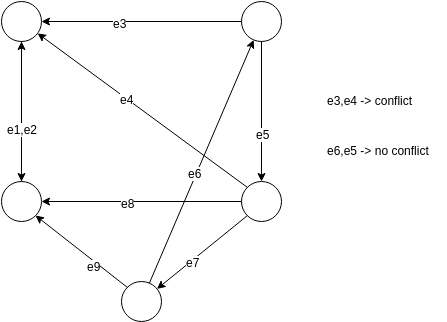
\includegraphics[width=0.6\textwidth]{head-partition}
	\caption{Head Partition Example}
	\label{fig:head-partition}
\end{figure}

\begin{minted}{Python}
# Algorithm 1
def headPartition(g):
  for node in g:
    select any incoming arc
\end{minted}

\begin{minted}{Python}
# Algorithm 2
# Version of "Generic Greedy Algorithm"
def headPartition2(g):
  edge_group = {}
  for arc in g.edges:
    if not conflict(arc, edge_group):
      edge_group += arc
\end{minted}

\end{document}
